\section{March 30, 2021} 
{\color{red}todo:brouwer stuff (not hard)} 

\subsection{Mod 2 degree: first attempt}
Fix a positive integer $n$. Let $X$ be a compact $n$-manifold and $Y$ a connected $n$-manifold. Suppose $f \colon X \to Y$ is smooth. If $q \in Y$ is a regular value, then $f ^{-1}(q)$ is a $0$-dimensional submanifold (by the preimage theorem). The degree counts the number of points in $f ^{-1}(q)$.
\begin{figure}[H]
\centering
 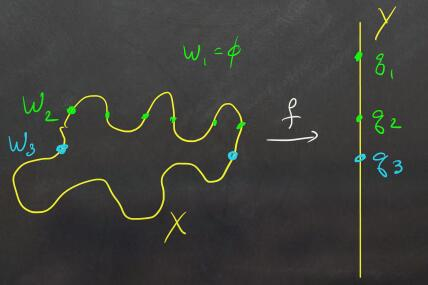
\includegraphics[width=0.5\linewidth]{figures/dtop_15.1.jpg}
 \caption{The mod 2 degree is independent of the regular value $q_i $.} 
 \label{mod2indp} 
\end{figure}
The standard degree depends on the regular value $q$; in \cref{mod2indp}, you can see the degree go from $0\to 6\to 2$ as $q_1\to q_2\to q_3$. However, mod 2 the degree is constant, so it's independent of $q$. Examine the inverse images $W_1$ and $W_2$ of the closed intervals $[q_1,q_2]$ and $[q_2,q_3]$; note that $W_1$ and $W_2$ are $1$-dimensional compact manifolds with boundary {\color{red}todo:see lec 13 for proof}. In fact, $W_1$ is a bordism from $f^{-1}(q_1)$ to $f^{-1}(q_2)$, while $W_2$ is a bordism from $f^{-1}(q_2)$ to $f^{-1}(q_3)$. 

The fact that this degree mod 2 is invariant follows from {\color{red}todo:see classificaiton of $1$-manifold lec: number of boundary points of a compact $1$-manifold is even}. As $t$ varies through $[q_1,q_3]$, we can see the birth and death of preimage pairs as we pass through critical values. 

\begin{definition}[]
    A \textbf{smooth homotopy} of maps $X \to Y$ between manifolds (without boundary) is a smooth map $F \colon [0,1] \times X\to Y.$ We write $F_t \colon X \to Y$ for the restriction of $F$ to $\{t\} \times X$.
\end{definition}

\begin{theorem}
    Fix $n \in \Z^{>0}$ and let $X$ be a compact $n$-manifold, $Y$ a connected $n$-manifold, and $f \colon X \to Y$ a smooth map. Then 
    \begin{enumerate}[label=(\arabic*)]
    \setlength\itemsep{-.2em}
\item The mod 2 cardinality $\# f^{-1}(q)\pmod 2$ of the inverse image of a regular value $q \in Y$ is independent of $q$.
\item If $F \colon [0,1] \times X \to Y$ is a smooth homotopy of maps, and $q \in Y$ a simultaneous regular value of $F,F_0,$ and $F_1$, then $\#F_0^{-1}(q)\equiv \# F_1^{-1}(q)\pmod 2$.
    \end{enumerate}
\end{theorem}
\begin{proof}
    For (2), note that the simultaneous regular values of $F,F_0,F_1$ exist by Sard's theorem. Observe that $\partial ([0,1]\times X)=\{0\} \times X \amalg \{1\} \times X$, so $\partial F=F_0 \amalg F_1$. {\color{red}todo:by some theorem}, we have $W:= F^{-1}(q)$ a $1$-dimensional submanifold of $[0,1]\times X$, and \[
        \partial W=W\cap (\{0\} \times X)\amalg W \cap (\{1\} \times X)=\{0\} \times F_0^{-1}(q)\amalg \{1\} \times F_1^{-1}(q).
    \] Since $\# \partial W$ is even, it follows that $\# F_0^{-1}(q)\equiv F_1^{-1}(q)\pmod 2$.
\end{proof}

{\color{red}todo:finish} 
\subsection{The mod 2 winding number}
Let $A$ be $(n+1)$-dimensional affine space with $V$ acting on $A$ by translations, $X$ be a compact $n$-manifold. Let $f \colon X \to A, q \in A \setminus f(x)$. Define $w_q \colon X \to S=S(v) \subseteq V, p \mapsto  \frac{f(p)-q}{\|f(p)-q\|}$. 
\begin{definition}
    The \textbf{mod 2 winding number} is given by \[
        W_2(f_1 q)=\deg_2 w_q \in \Z /2\Z.
    \] 
\end{definition}
\begin{remark}\,
    \begin{itemize}
        \setlength\itemsep{-.2em}
        \item $w_2(f,q)$ depends only on $[q] \in \pi_0(A \setminus f(x))$,
        \item $w_2(f,q)$ is unchanged under smooth homotopies of $f$ which do not contain $q$ in the image.
    \end{itemize}
\end{remark}
There are two methods to compute $w_2(f,q)$.
\begin{theorem}
    If $W$ is a compact $(n+1)$-manifold with $\partial W=X$, $F \colon W \to A$ such that $\partial F=f$, suppose $q \in A \setminus f(X)$ is a regular of $F$. Then $w_2(f,q)=\# F^{-1}(q) \pmod 2$.
\end{theorem}
\begin{proof}
    {\color{red}todo:free time} 
\end{proof}
\begin{theorem}
    Let $z=z_q(\xi)$. If $f\transv z$, then $w_2(f,q)=\#_2(f,z)$ in $Y=A \setminus \{q\} $.
\end{theorem}

\subsection{The Jordan Brouwer theorem}
This is the famous topological fact that's notoriously hard to prove. Say we embed $S^1 $ in $\R^2$. Then the embedding has two components, a bounded interior and an unbounded exterior.
\begin{namedthm}{The Jordan curve theorem} 
    Suppose $X \subseteq A$ (where $A$ is affine space) is a compact connected hypersurface (submanifold of codimension 1). Then $A \setminus X$ has two path components $D_0,D_1$, exactly one of which, say $D_1$, is bounded. The closure $\overline{D_1}$ is a compact manifold with boundary with $\partial \overline{D_1}=X$. Finally, if $q \in D_j $, then $w_2(i_X,q)=j\pmod 2$, where $i_x \colon X \to A$ denotes the inclusion.
\end{namedthm}
\begin{proof}
    {\color{red}todo:} 
\end{proof}
Seems like Borsuk Ulam is going in the notes.
\begin{cor}
    There does not exists an embedding $\R \mathrm P^2 \hookrightarrow \A^3$.
\end{cor}
